Table \ref{tab:assumptions} contains some assumptions and approximations about the working conditions and applied loads.

\begin{table}[H]
    \centering
    \caption{Assumptions Made During Robot Modelling}
    \label{tab:assumptions}
    \begin{tabular}{l l}
        \\ \hline
        \textbf{Assumption Type} & \textbf{Assumption} 
        \\ \hline
        Hip Range of Motion & 0\textdegree{} (horizontal) to 30\textdegree{}
        \\
        Knee Range of Motion & Foot no further inwards than knee
        \\
        Maximum wind speed & 73 km/h (Ottawa, September 2018 Tornadoes)
        \\
        Linkage composition & Homogeneous rigid bodies
        \\
        Terrain & Sand, pebble, shallow water (under chassis), mud, small plants
        \\
        Environment & Salt, dust, high heat, humidity
        \\ \hline
    \end{tabular}
\end{table}

The first two assumptions relate to the mechanical stability of the robot. It is more stable when the body is closer to the ground, and when it has a wider base.
The first assumption stipulates that, during operation, the hip joint will allow the thigh to turn between horizontal and 30 degrees above horizontal, keeping the body lower than if a negative angle was selected.
The second states that the foot will extend beyond the thigh, but will never retract closer than the knee, since it will require more torque to counter-balance an external force, making it less stable.
A maximum value was selected for wind speed based on Ottawa peak wind speeds (including the tornado events). It is assumed that the robot would not be left operating in more extreme weather, such as hurricanes.
Other assumptions are based on basic simplification of the calculations or on the given requirements.


\subsection{Tibia Simplification During Analysis}

As seen in the concept image in Figure \ref{fig:crab_leg}, the tibia linkage is to have a bend. This will help reduce the angle at the knee for the bellows. However, for the force analysis, the shin was simplified as a simple line joining each end of the member. This is shown as the dashed line in Figure \ref{fig:robot_leg_assumption}. 

\begin{figure}
    \centering
    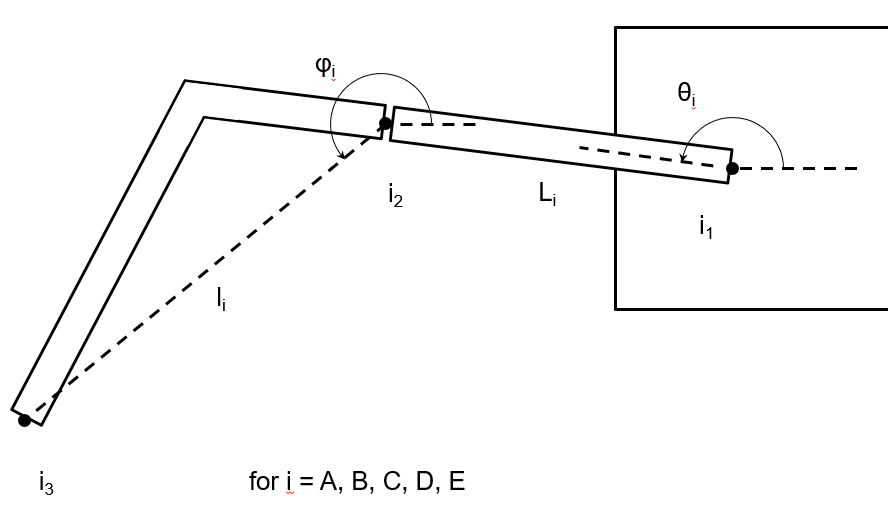
\includegraphics[width=\textwidth]{4_ComponentProperties/img/robot_leg_assumption.PNG}
    \caption{Crab Straight Leg Assumption}
    \label{fig:robot_leg_assumption}
\end{figure}

\subsection{Friction}

The friction force is shown in all FBDs. However, in the calculations without slope, these were assumed to be negligible compared to the normal forces at the feet. 
The friction forces only comes into effect when the robot is on a slope. However, the calculated slope in terms of stability is relatively small and thus friction is assumed to have little impact in this case. This assumption is further supported by the fact that the robot legs will dig into the sand, mud or pebbles to a certain extent. This would create additional normal forces on the side of the foot, preventing the robot from slipping easily.

\subsection{Nominal and Actual Values for Motors}
\label{sec:ass_motors}

The approximate weights and power usage of the motors were inspired by existing harmonic drive and motor models. The characteristics of the observed models are shown in Tables \ref{tab:motors} and \ref{tab:HDs}, and datasheets are included in Appendix \ref{app:data_sheets}\cite{harmonic_drive_csd-2a_nodate} \cite{maxon_motor_ec60_nodate}.

\begin{table}[H]
    \centering
    \caption{Motors Used for Power and Weight Approximations}
    \label{tab:motors}
    \begin{tabular}{l c c}
        \\ \hline
        \textbf{Properties} & \textbf{Hip Motor} & \textbf{Knee Motor}
        \\ \hline
        Manufacturer & Maxon & Maxon
        \\
        Model & EC 90 Flat & EC 60 Flat
        \\
        Weight [kg] & 0.98 & 0.36
        \\
        Diameter [mm] & 90 & 60 
        \\
        Voltage [V] & 48 & 48
        \\
        Nominal Current [A] & 4.06 & 4.6
        \\
        Nominal Torque [mNm] & 964 & 577
        \\
        Stall Torque [Nm] & 13.1 & 4.87
        \\ \hline
    \end{tabular}
\end{table}

\begin{table}[H]
    \centering
    \caption{Harmonic Drives Used for Power and Weight Approximations}
    \label{tab:HDs}
    \begin{tabular}{l c c}
        \\ \hline
        \textbf{Properties} & \textbf{Hip Harmonic Drive} & \textbf{Knee Harmonic Drive}
        \\ \hline
        Manufacturer & Harmonic Drive & Harmonic Drive
        \\
        Model & FB-40-100-2-GR & 	FB-25-100-2-GR 
        \\
        Reduction Ratio & 100 & 100
        \\
        Weight [kg] & 1.8 & 0.5 
        \\
        Diameter [mm] & 135 & 85 
        \\
        Rated Torque [Nm] & 157 & 39
        \\
        Average Torque Limit [Nm] & 186 & 52
        \\
        Momentary Peak Torque [Nm] & 343 & 91
        \\ \hline
    \end{tabular}
\end{table}

Calculations were based when possible on nominal or rated torque values, to make them correspond to the calculated moments at the joints. However, as this analysis takes into account the worse case scenarios for the robot, it must be understood that the motors will not always be operating at their nominal point. These occurrences would happen on rare or momentary occasions. Thus, in those cases the average torque limit or momentary peak torque are considered.
The harmonic drives FB-series are also non-backdrivable; when the robot is stationary, the harmonic drives will take the static torque, significantly reducing the power drawn from the motors.